\documentclass{standalone}
\usepackage{tikz}
\usetikzlibrary{arrows.meta}

\begin{document}
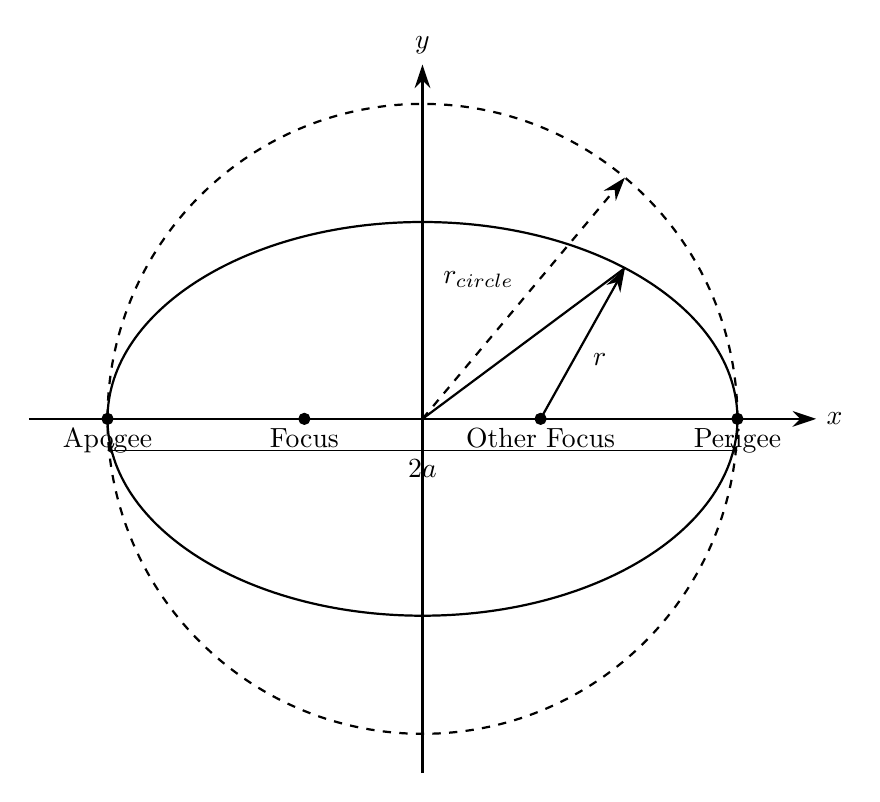
\begin{tikzpicture}

% Define some parameters
\def\a{4}  % semi-major axis
\def\b{2.5}  % semi-minor axis
\def\focus{1.5}  % distance from center to focus
\def\angleE{50}  % eccentric anomaly angle
\def\circumradius{\a}  % radius of the circumscribing circle (same as the semi-major axis)

% Draw ellipse
\draw[thick] (0,0) ellipse (\a cm and \b cm);

% Draw major and minor axes with Stealth arrowheads, extended to fit the circle
\draw[thick, -{Stealth[length=3mm, width=2mm]}] (-\a-1,0) -- (\a+1,0) node[anchor=west] {$x$};
\draw[thick, -{Stealth[length=3mm, width=2mm]}] (0,-\circumradius-0.5) -- (0,\circumradius+0.5) node[anchor=south] {$y$};

% Draw focus points
\filldraw[black] (-\focus,0) circle (2pt) node[anchor=north] {Focus};
\filldraw[black] (\focus,0) circle (2pt) node[anchor=north] {Other Focus};

% Draw apogee and perigee
\filldraw[black] (-\a,0) circle (2pt) node[anchor=north] {Apogee};
\filldraw[black] (\a,0) circle (2pt) node[anchor=north] {Perigee};

% Draw line from the focus to a point on the ellipse
\draw[thick, -{Stealth[length=3mm, width=2mm]}] (\focus,0) -- ({\a*cos(\angleE)},{\b*sin(\angleE)}) 
   node[midway, anchor=north west] {$r$};

% Draw angle at the focus
\draw[thick] (\focus,0) -- (0,0);
\draw[thick] (0,0) -- ({\a*cos(\angleE)},{\b*sin(\angleE)});
\draw[dashed] (-\focus,0) -- ({\a*cos(0)},{\b*sin(0)});

% Draw line from the origin to the corresponding point on the circumscribing circle
\draw[thick, dashed, -{Stealth[length=3mm, width=2mm]}] (0,0) -- ({\circumradius*cos(\angleE)},{\circumradius*sin(\angleE)}) 
   node[midway, anchor=south east] {$r_{\text{circle}}$};

% Label the semi-major axis
\draw[<->] (-\a, -0.4) -- (\a, -0.4) node[midway, anchor=north] {$2a$};

% Draw the circumscribing circle
\draw[thick, dashed] (0,0) circle (\circumradius);

\end{tikzpicture}
\end{document}
